% Orla comments 20-Dec04
% Ian comments 20-Dec04
% TO BE UPDATED with latest pictures of the environment
% TODO: Dominic comments 20-Dec04

\ifx\wholebook\relax\else
\input{../Common.tex}
\input{../macroes.tex}
\begin{document}
\fi
	
\chapter{Getting Started}\label{ch:firstcontact}

The purpose of this chapter is that in five minutes from now you can be ready to use the environment you will use in this book. In this chapter you will learn how to install the  environment, understand the different parts of the environment and how to interact with the robots that live in this environment. You shall program these robots to accomplish challenging tasks by sending them messages.

Right now we just want to get you started and get ready for the rest of the book.   Note that if your environment is already installed then simply jump directly to the subsequent sections that explain the environment. Chapter~\ref{cha:caroTour} will explain in more detail the environment. 


%%%%%%%%%%%%%%%%%%%%%%%%%%%%%%%%%%%%%%%%%%%
\section{Installing the Environment}
The environment used in this book is developed on top of \sq. \sq is a rich and powerful open-source multimedia environment entirely written in Smalltalk and freely available for most of the computer and operating systems at http://www.\-squeak.\-org. Note however that you will not use directly a default  \sq distribution but use instead a distribution I prepared for you.  

\sq runs exactly the same on all the platforms, however to ease your start we prepared some platform dependent compressed files. The principle is exactly the same on Mac, PC, or any other platforms. Only the decompressing tools and the way to invoke \sq may differ. Once you have a file named \ct{ReadyToUse.zip}, you decompress it then drag the file named \ct{Ready.image} on the \ct{Squeak application}, and this is it! The file \ct{Ready} contains the complete environment used in this book

Now let us look at each of the steps one by one. Note that you may get files with slightly different names but it should work exactly the same.

\paragraph{On Macintosh.}
You should have a file named  \ct{readyToUseForMac.zip} a zipped archive. Normally double-clicking on the file should invoke the right decompresser such as StuffIt Expander. When you decompressed this file, you should obtain 4 files as shown by Figure~\ref{fig:macfiles}. You should identify two files: the file named \ct{Ready.image} and the \emph{Squeak application} file (the one without extension in Figure~\ref{fig:macfiles} it is named \ct{Squeak}).

\begin{figure}[h]\centerline{\includegraphics{readyToUseMacZip2}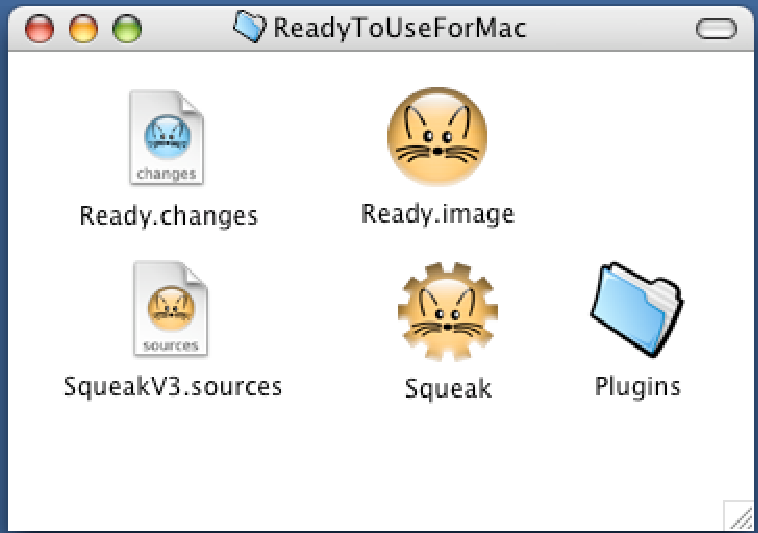
\includegraphics[width=9cm]{macFiles2}}
\caption{The files for the ready to use environment for Macintosh. Left: the zipped file. Right: the files.\label{fig:macfiles}}\end{figure}


\newpage


\paragraph{On Windows.}
You should have a file named \ct{readyToUse.zip}, an archive.  When you decompressed this file using Winzip, you should obtain 4 files as shown by Figure~\ref{fig:pcfiles}. You should identify two files: the file named \ct{Ready.image} and the \emph{Squeak application} file (the one without extension in Figure~\ref{fig:pcfiles} it is named \ct{Squeak}.


\begin{figure}[h]\centerline{
\includegraphics{zipPC}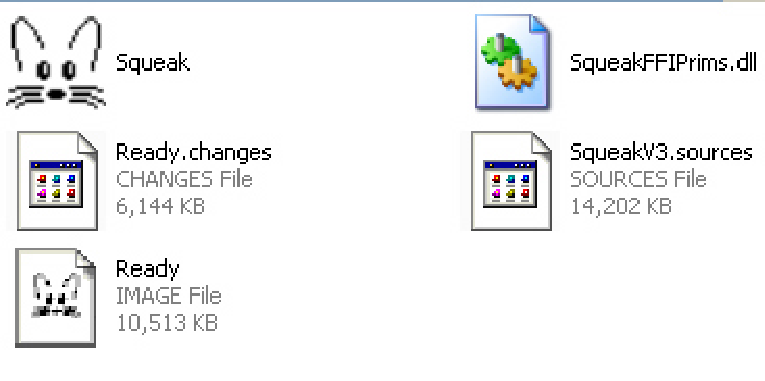
\includegraphics[width=9cm]{readyPC}} 
\caption{The files for the ready to use environment on PC. Left: the zipped file. Right: the files.\label{fig:pcfiles}}
\end{figure}


\section{Opening the Environment} 
To open the environment, drag the file \ct{Ready.image} on the \emph{Squeak application} that is the file named Squeak as shown by Figure~\ref{fig:dropImage}. You should get the environment shown in Figure~\ref{fig:firstEnvironment}. If you do not get this environment then read Section~\ref{sec:trouble}.

\begin{figure}[!h]\centerline{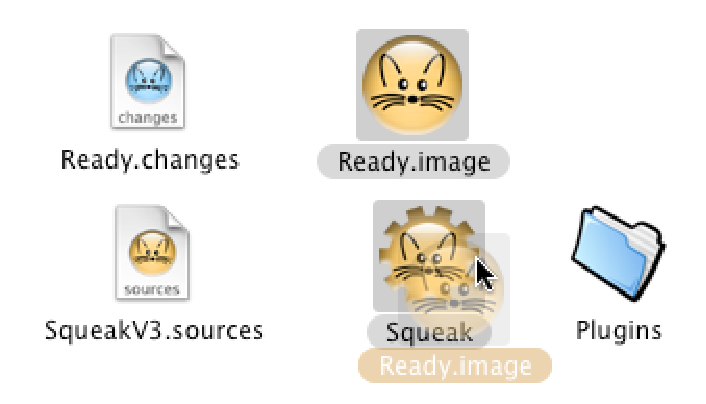
\includegraphics[width=8cm]{dropImage2}  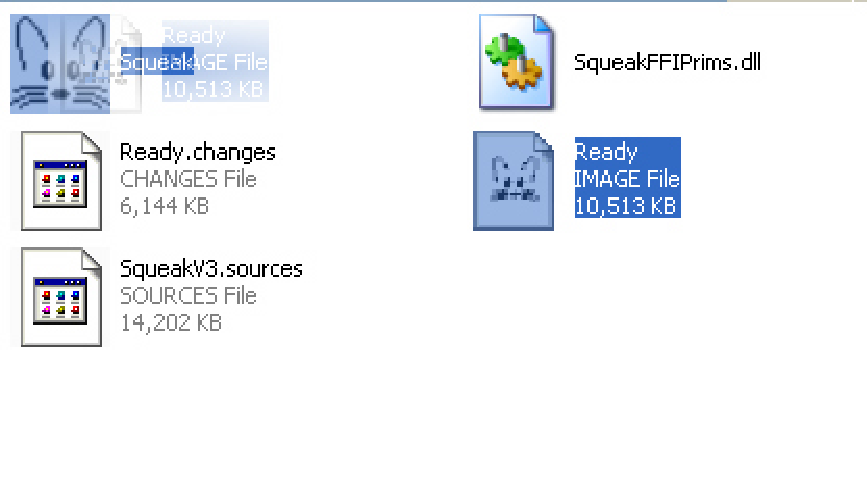
\includegraphics[width=8cm]{readyDD}} 
\caption{Dragging and dropping the \textit{image} file on the 
\textit{Squeak application} to open on Mac (left) on PC (right).\label{fig:dropImage}}
\end{figure}

\paragraph{Hints.}
The environment can be opened by simply double-clicking on the \textit{image} file. However, such a practice has several disavantages: you may have to identify the \emph{Squeak application} and sometimes another application may by accident try to use the image. Moreover it can lead you to trouble when you have multiple installations of different versions of \sq. So we suggest to always open the environment by dragging and dropping the \emph{image file} on the \emph{Squeak application} file or alias to it. Note that if you have space problem you can use an alias to the SqueakV3.sources file as this file can be shared between multiple installations. 

\begin{largecadre}{To start the environment. 
Drag and drop the file terminating with the .image extension into the squeak application.}
\end{largecadre}
 
%%%%%%%%%%%%%%%%%%%%%%%%%%%%%%%%%%%%%%%%%%%
\section{First Interactions with a Robot}

Once you open the environment by dragging the file named \ct{Ready.image} on the Squeak executable as explained previously, you should obtain an environment similar to the one presented by Figure~\ref{fig:firstEnvironment}. 


\begin{figure}[!h]\centerline{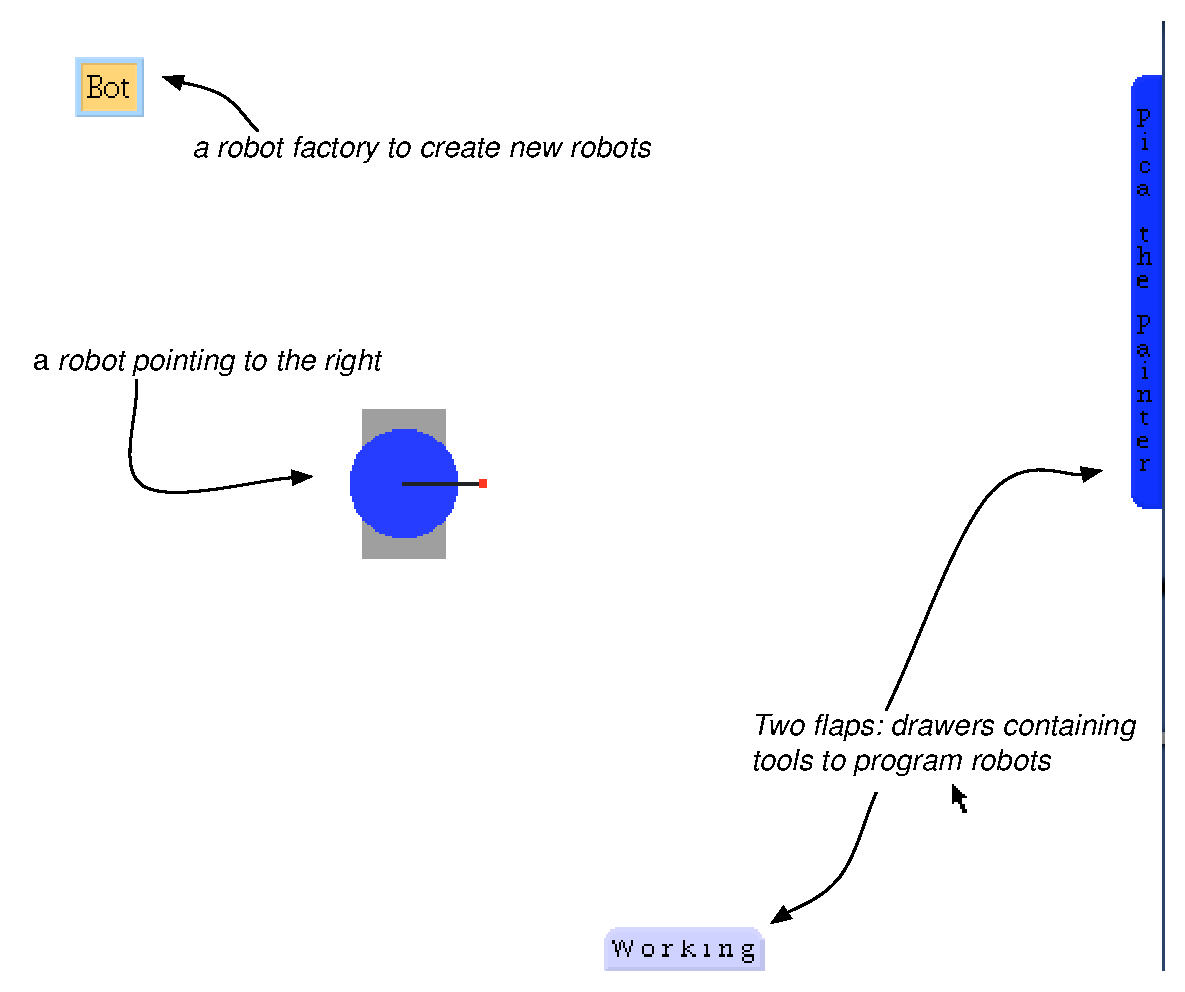
\includegraphics[width=10cm]{firstEnvironmentAnnotated}} 
\caption{The environment ready to use.\label{fig:firstEnvironment}}
\end{figure}

The environment is composed of robot factories and two flaps. A flap is a drawer containing programming tools that you do not need to use now and we will describe later in Chapter~\ref{cha:caroTour}. Now you should see a small blue robot in the middle of the screen. Of course this is not a physical robot, but a software robot seen from above pointing on the right of the screen.  A robot is a round blue circle; it has two catterpilars and a small red head indicating its current direction. In this book you shall send orders to robots, we say that we send them \emph{messages} \index{messages} and robots execute these messages.

Place the mouse over the robot and wait a second there. A balloon pops up with some information about the robot such as its current location and its direction as shown in Figure~\ref{fig:firstBalloon}. As your screen is of different size than the one used to produce this book, you may have other values.  

\begin{figure}[!h]\centerline{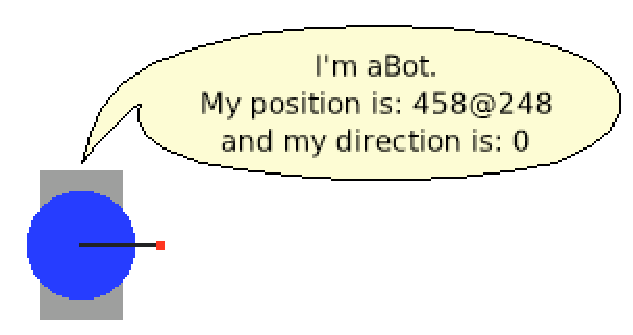
\includegraphics[width=8cm]{firstBalloon2}}
\caption{Place the mouse over a robot to get a balloon showing some information related to the robot in question.\label{fig:firstBalloon}}
\end{figure}

\paragraph{Sending Messages to a Robot.}
To interact directly with a robot by left-clicking on the robot with the mouse.  A messaging balloon pops up as shown by the left picture of Figure~\ref{fig:go}.  You can type some messages that are sent to the robot. Once you typed these messages, hitting the \bold{return} key actually sends them to the robot which will then execute them.

\begin{figure}[h]\centerline{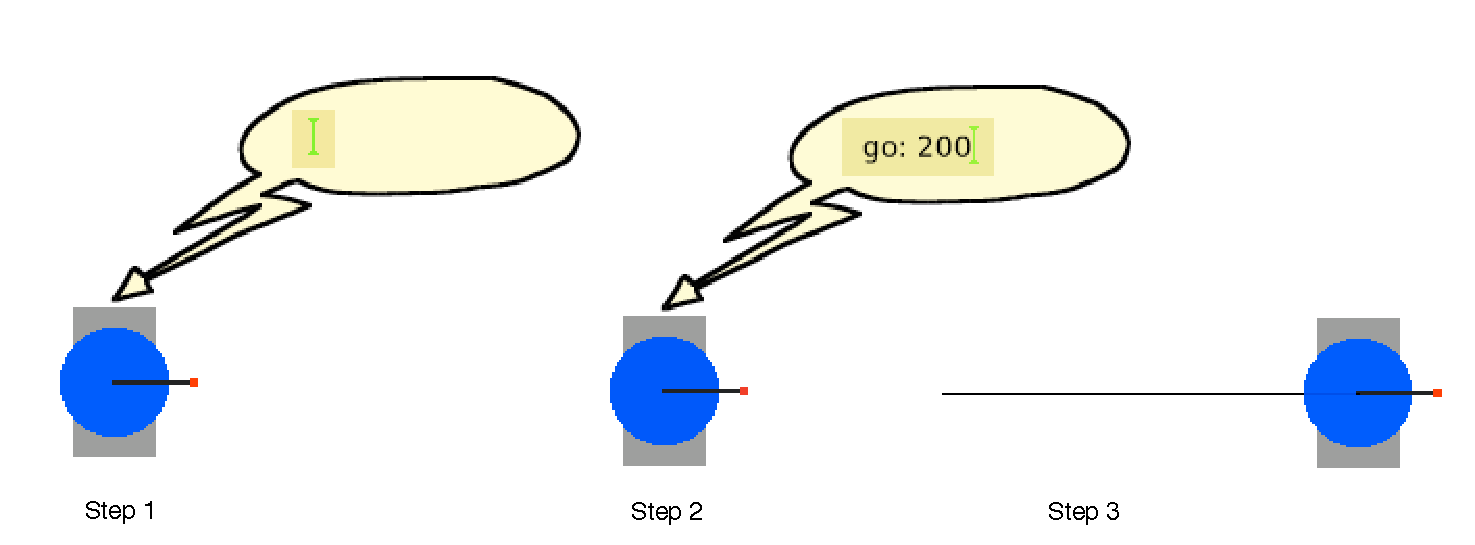
\includegraphics[width=16cm]{sendingAMsg2}}
%emptyBalloon}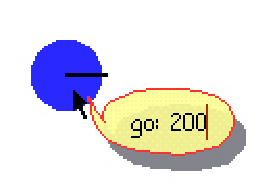
\includegraphics{go}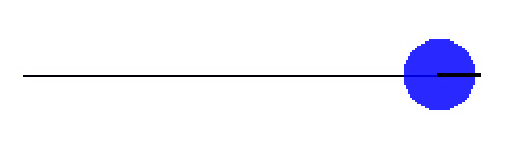
\includegraphics{gone}}
\caption{Step 1: left-clicking on a robot produces a balloon to send a message to a robot. Step2: Typing a message to ask a robot to move forward. Step 3: the robot moved and left a trace on the ground.\label{fig:go}}
\end{figure}

\begin{figure}[!h]\centerline{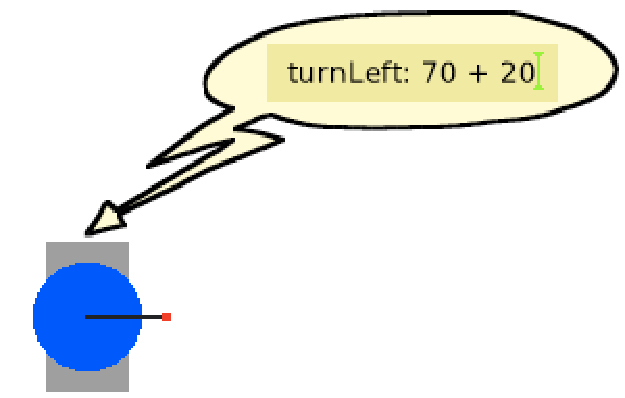
\includegraphics{turn20+702}\hfill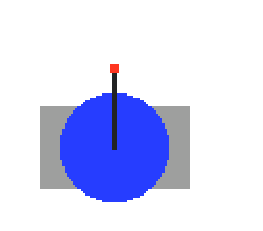
\includegraphics{turned2}}
\caption{Left: Sending a complex message. Right: Its effect.\label{fig:turned}}
\end{figure}

 For example by typing the message \ct{go: 200} and hitting the return key, we ask the robot to move forward 200 pixels in its current direction, or typing the message \ct{turnLeft: 20 + 70} we ask the robot to turn on its left of 90 degrees. The message \ct{color: Color green} changes the color of the robot as shown by the Figure~\ref{fig:green}.

As the messages show, we can write complex messages and we will explain how you can write such messages later. For now simply type what we show you. Note that if you want to repeat some expressions, you do not have to retype them but simply use the up and down arrows to navigate over the previous messages you sent to the robot. In the subsequent chapters, you shall learn step by step all the messages that a robot understands and more important you shall learn how to define new behavior for your robots.





\begin{figure}[!h]\centerline{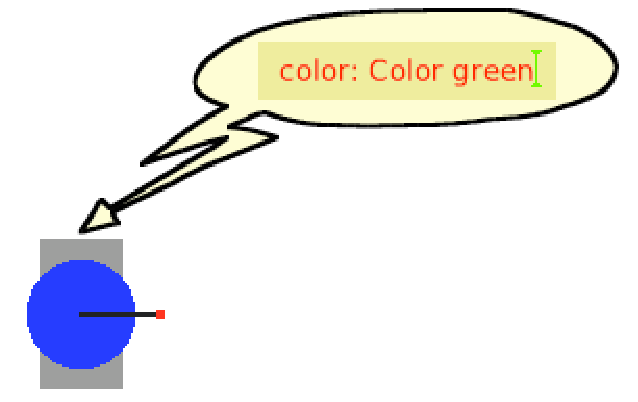
\includegraphics{colorGreen2} \hfill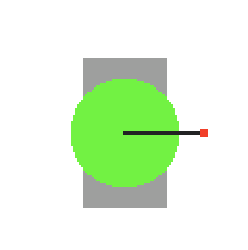
\includegraphics{green2}}
\caption{Left: Changing the color of a robot to another color. Right: its effect \label{fig:green}}
\end{figure}


\begin{largecadre}{To interact with a robot. Click on it, type the message and hit the \bold{return} key.}
\end{largecadre}

%%%%%%%%%%%%%%%%%%%%%%%%%%%%%%%%%%%%%%%%%%%
\section{Creating a New Robot}
The environment already contains a robot but now we show you how to create new robots. To create a new robot we ask a robot \emph{factory} to create a new one. A robot factory is graphically represented by an orange box surrounded by a blue light box in the middle of which the word Bot is written as shown in Figure~\ref{fig:classBalloon}. A robot factory \index{robot factory} is called in \sq jargon a \index{class} \emph{class}.
Classes (object factories) have a name starting with an uppercase letter. Hence this is the class \ct{Bot} and not \ct{bot}.  

As for robots, we interact with a robot factory by sending it messages. The message to create a new robot is the message \ct{new} as shown in Figure~\ref{fig:turtleBoxNew}. 
Note that newly created robots point also to the right of the screen. Now you can send messages to the two robots individually, each of them living its own life. 

\begin{figure}[!h]\centerline{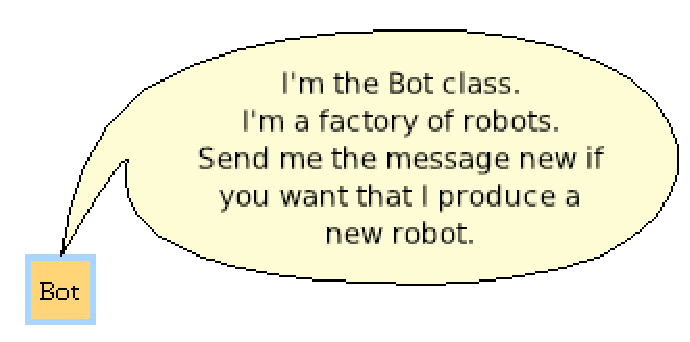
\includegraphics[width=8cm]{classBalloon2}}
\caption{A robot factory called in \sq jargon a \emph{class}. It produces new robots. \label{fig:classBalloon}}
\end{figure}

\begin{figure}[!h]\centerline{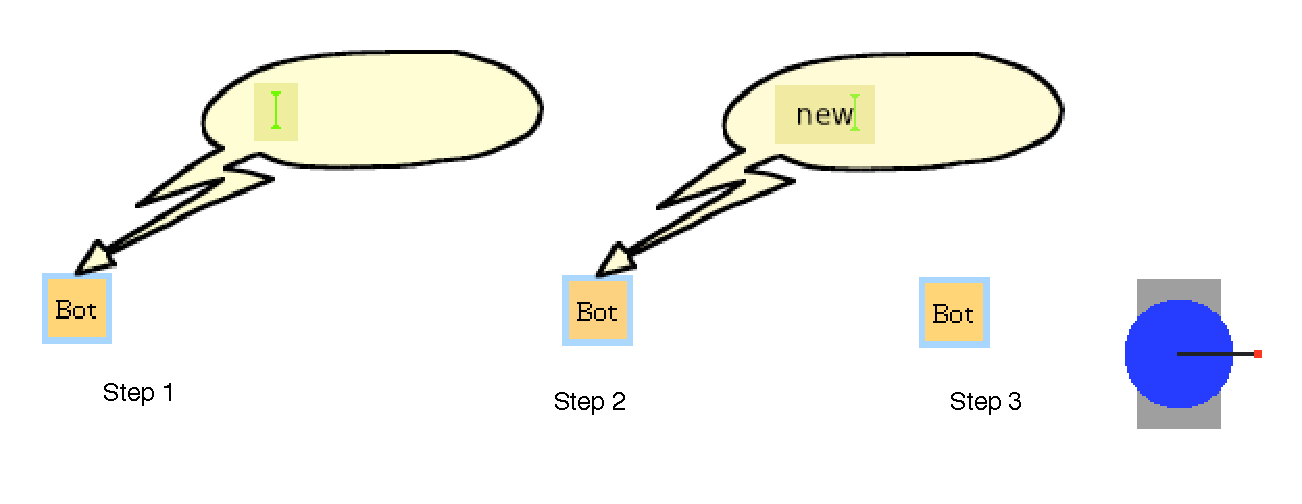
\includegraphics[width=14cm]{creatingARobot2}}
%{turtleBoxNew} 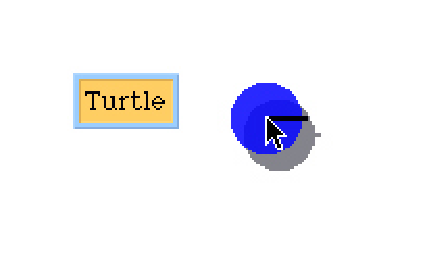
\includegraphics{newTurtleInHand}}
\caption{Step 1: Start to type a message. Step 2: sent the message \ct{new} to the factory to get a new robot. Step3: The factory creates a robot and gives it to you.\label{fig:turtleBoxNew}}
\end{figure}

\begin{largecadre}{To create new robots. Send the message \ct{new} to the robot factory, a class.}
\end{largecadre}

When a robot is created, it is always pointing to the east or the right of the screen. 


%\section{Getting an Animated Robot}
%The robot with which you just interacted was not animated \ie you could not see how the messages were performed. Sometimes it would be nice to see the robot executing the messages step by step. This is possible. For this you have to create an animated robot by sending the message \ct{new} to the class \ct{AniBot} as you did previously to get new robots. The new robot you get understands all the messages a basic robot understands. 
%Animated robots are green to distinguish them from basic ones. Send some messages to the robot to see it performing them.

%\begin{figure}[!h]\centerline{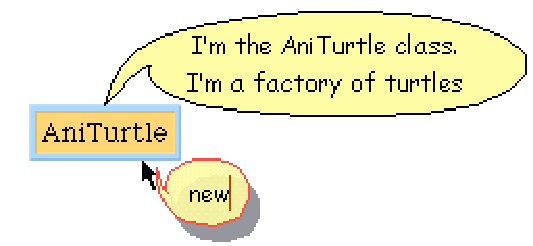
\includegraphics{aniTurtleClassNew}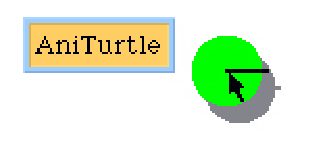
\includegraphics{aniTurtle}}
%\caption{Left: Asking the animated robot factory to create a new robot. Right: Getting a new animated robot. \label{fig:animated2}}
%\end{figure}

%%\begin{figure}[!h]
%%\begin{center}
%%\centerline{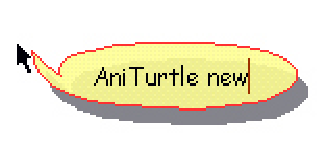
\includegraphics{aniTurtleNewInBalloon}}
%%\caption{Creating an animated turtle.\label{fig:animatedcreated}}
%%\end{center}
%%\end{figure}

%Note that if the animation speed is too slow you can change it using the message \ct{speed:} and providing a number such as 1000 or 10000. For example, type in the balloon \ct{speed: 10000} to test it.  



%%%%%%%%%%%%%%%%%%%%%%%%%%%%%%%%%%%%%%%%%%%
\section{Quitting and Saving}\label{sec:quit}

The background of the \sq window application is called the \index{world} World. The World has a menu offering a lot of functionality. To display the World menu just click on the background. You should get a menu similar to the one shown in Figure~\ref{fig:worldMenu}. The last group of elements are all the actions you can do to quit or save your work. 

\begin{figure}[!h]
\center{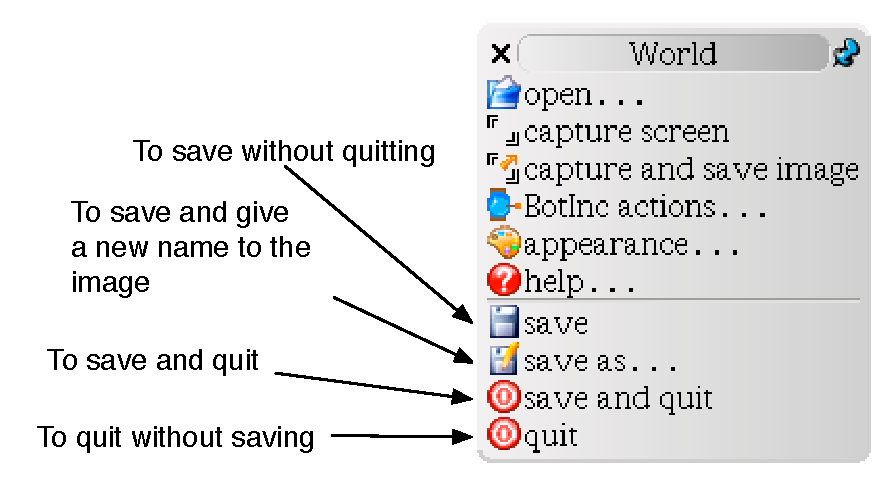
\includegraphics[width=8cm]{worldMenuAnnotated}}
\caption{The World menu.\label{fig:worldMenu}}
\end{figure}

Selecting the item 'quit' simply quit without saving what you did. Therefore the next time that you will restart the environment it will be exactly in the same state as when you started this time. Selecting the item 'save', save the complete environment. The next time you till start it, it will be exactly in the same time that at the moment you saved it. 
Finally when selecting the item 'save as...',  the environment asks you to give a new name and it will create two new files with that name: one with the extension \ct{.image} and one with the extension \ct{.changes}.  This is this way that we created the files \ct{Ready.image} and \ct{Ready.changes}.  To open the environment you saved with a new name, drag and drop the file with the new name which has the extension \ct{.image} on the squeak executable as you did to start the environment by dragging and dropping the file \ct{Ready.image}.





\section{Possible Installation Troubleshootings}\label{sec:trouble}
Now we try to help to fix the problems you may encounter during the installation. For that we will explain the role of each important files you got once you decompressed the archive.

To run the environment provided with this book or any  \sq distribution, four files are necessary. We describe them now as we will use their name to help solve the possible problems you may encounter.  The four files are: 
\begin{description} 
\item[Image and changes.] The file named \ct{Ready.image}, called simply the \textbf{image}\index{image file} file and the file named \textbf{Ready.changes}, called simply the \textbf{changes} \index{changes files} file contain the information of your current system. These two files are synchronized by \sq automatically and \emph{should be writable}. Each time you save you environment they are synchronized. You should not edit then with another file editor or changes the name of the file manually. If you want to have different names, just use the \menu{save as ...}
menu item of the World menu, \sq will then create a new pair of files for you. 

 
\item[Source.] The file named \ct{SqueakV3.sources}, also called \textbf{sources}\index{sources file}, contains the source of a part of the \sq environment. You do not need it in this book so do not try to edit manually. However, this file should always be in the directory in which the image is.
  
\item[Application.] The application Squeak for mac or Squeak.exe for PC is the \sq system. This is this application that runs when you program in \sq. It should then be executable. We refer to this file as the \index{Squeak application}\textbf{Squeak application}. In computer scientist jargon, this application is called a \index{virtual machine} virtual machine called or  a VM \index{VM} in short. 
\end{description}

As we already mentioned it the \textit{image} and \textit{changes} files should be writable. Certain operating systems change the properties of the files to read-only when copied from a CD. In such a case, \sq warns you with a message as shown in Figure~\ref{fig:readonlyfile}. If you get this message, simply quit \sq without saving, change the property of the file to be writable and restart.  

\begin{figure}[!h]\centerline{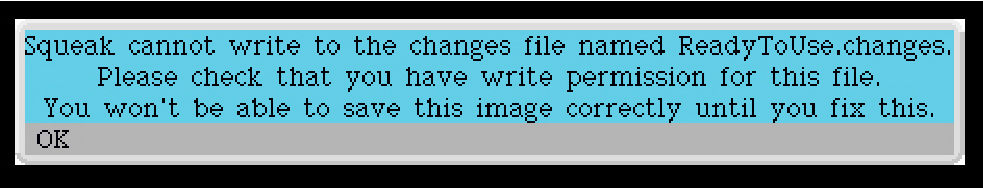
\includegraphics[width=\linewidth]{changesNotWritable}}\caption{The error message showing that
 the image (\ct{Ready.image}) or changes (\ct{Ready.changes}) files are not writable.\label{fig:readonlyfile}}
\end{figure}

Another possible problem you may encounter is related to the sources file named \ct{SqueakV3.sources}, this file or an alias to this file should be present in the directory where the image file is. When this file is not present you may get on Mac the first message shown in Figure~\ref{fig:sourcesMissing} (note that this message is not clear and refers to a problem related to aliases that is fixed in the current version of \sq) or the second message. To cure this problem, create an alias to the source file (\ct{SqueakV3.sources}) into the directory containing  your image or simply copy the sources file  to be in the same directory that the image file.

\begin{figure}[!h]%\center{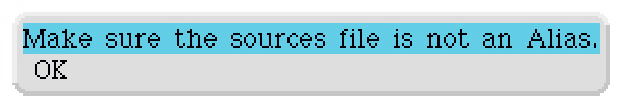
\includegraphics{sourcesMissing}}
\center{\includegraphics[width=\linewidth]{sourcesMissing2}}\caption{Some possible error messages indicating that the \textit{source} file (\ct{SqueakV3.sources}) is missing in the directory containing the \textit{image} file .\label{fig:sourcesMissing}}
\end{figure}





%%%%%%%%%%%%%%%%%%%%%%%%%%%%%%%%%%%%%%%%%%%
\summa

\begin{itemize}
\item To start the environment, drag and drop the file terminating with the .image extension into the squeak application.

\item To send a message to a robot, left-click on it, type the message and hit the \bold{return} key.

\item To create new robots. Send the message \ct{new} to the robot factory, a class.
%\item  In an interaction balloon the word \ct{self} refers to the robot receiving the message.

\item When a robot is created, it is always pointing to the east or the right of the screen. 

\item The background of the environment is called the World.

\item To get the menu to save the environment, click on the background close to a robot.
\end{itemize}



\ifx\wholebook\relax\else\end{document}\fi



